\documentclass[11pt]{article}


    \usepackage[breakable]{tcolorbox}
    \tcbset{nobeforeafter} % prevents tcolorboxes being placing in paragraphs
    \usepackage{float}
    \floatplacement{figure}{H} % forces figures to be placed at the correct location
    \usepackage{multicol}
	\usepackage[english]{babel}
    \usepackage{tabularx}
    \usepackage{subfigure}
    \usepackage{picture}
    \usepackage{amsmath}
    \usepackage{hyperref}
    \hypersetup{
    colorlinks=true,
    linkcolor=blue,
    filecolor=magenta,      
    urlcolor=cyan,
    }
    \usepackage{graphicx}    
    \usepackage{caption}
    \usepackage{adjustbox} % Used to constrain images to a maximum size 
    \usepackage{xcolor} % Allow colors to be defined
    \usepackage{enumerate} % Needed for markdown enumerations to work
    \usepackage{geometry} % Used to adjust the document margins
    \usepackage{amsmath} % Equations
    \usepackage{amssymb} % Equations
    \definecolor{urlcolor}{rgb}{0,.145,.698}
    \definecolor{linkcolor}{rgb}{.71,0.21,0.01}
    \definecolor{citecolor}{rgb}{.12,.54,.11}
    

    
    % Prevent overflowing lines due to hard-to-break entities
    \sloppy 
    % Setup hyperref package
    \hypersetup{
      breaklinks=true,  % so long urls are correctly broken across lines
      colorlinks=true,
      urlcolor=urlcolor,
      linkcolor=linkcolor,
      citecolor=citecolor,
      }
    % Slightly bigger margins than the latex defaults
    
    \geometry{verbose,tmargin=1in,bmargin=1in,lmargin=0.4in,rmargin=1in}
    \usepackage{fancyhdr}
    \pagestyle{fancy}
    \renewcommand{\footrulewidth}{1pt}
    \rhead{e11921655 Fabian Holzberger \\ e01526208 Jan Ellmenreich}
    \lhead{VU\,184.725\\ High Performance Computing}
    \cfoot{\thepage}
    \setcounter{secnumdepth}{0}
    \setlength\parindent{0pt}

    \usepackage{booktabs}

    \usepackage{listings}
    \usepackage[linesnumbered,ruled,vlined]{algorithm2e}
    \newcommand\mycommfont[1]{\footnotesize\ttfamily\textcolor{blue}{#1}}
    \SetCommentSty{mycommfont}
    \SetKwInput{KwInput}{Input}                % Set the Input
    \SetKwInput{KwOutput}{Output}              % set the Output



\title{Exercise 0 Dataset description}
\author{e12045110 Maria de Ronde \\ eXXXXXXXX  Quentin Andre  \\ e11921655 Fabian Holzberger}
\date{\today}

\begin{document}
\graphicspath{{./figures/}}
\maketitle

\newpage
%
\section{Classification Dataset: Email-Spam (\href{https://www.kaggle.com/nitishabharathi/email-spam-dataset?select=enronSpamSubset.csv}{link to dataset})}


\section{Bridges Dataset(\href{https://archive.ics.uci.edu/ml/datasets/Pittsburgh+Bridges}{link to dataset})}





\section{Kaggle: Amazon review}
\subsection{Dataset Description} 
The Amazon review dataset is used to predict the author of reviews. The reviews are translated into vectors. There are 50 classes, which represent authors of different reviews. The dataset contains 750 instances with 100002 vectors, a nominal attribute representing a unique ID, 10000 numerical vectors and a nominal vector representing the class.
\newline 
In the figure \ref{Fig::Instances_per_class} one can see how many instances belong to each class. We can see that the dataset is unbalanced. As some classes have 20 instances where other classes have only 10 instances.
%
\begin{figure}[h]
%\begin{figure}[h]
%\begin{picture}(400,285)
\begin{minipage}[t]{0.8\textwidth}
%\put(0,0){
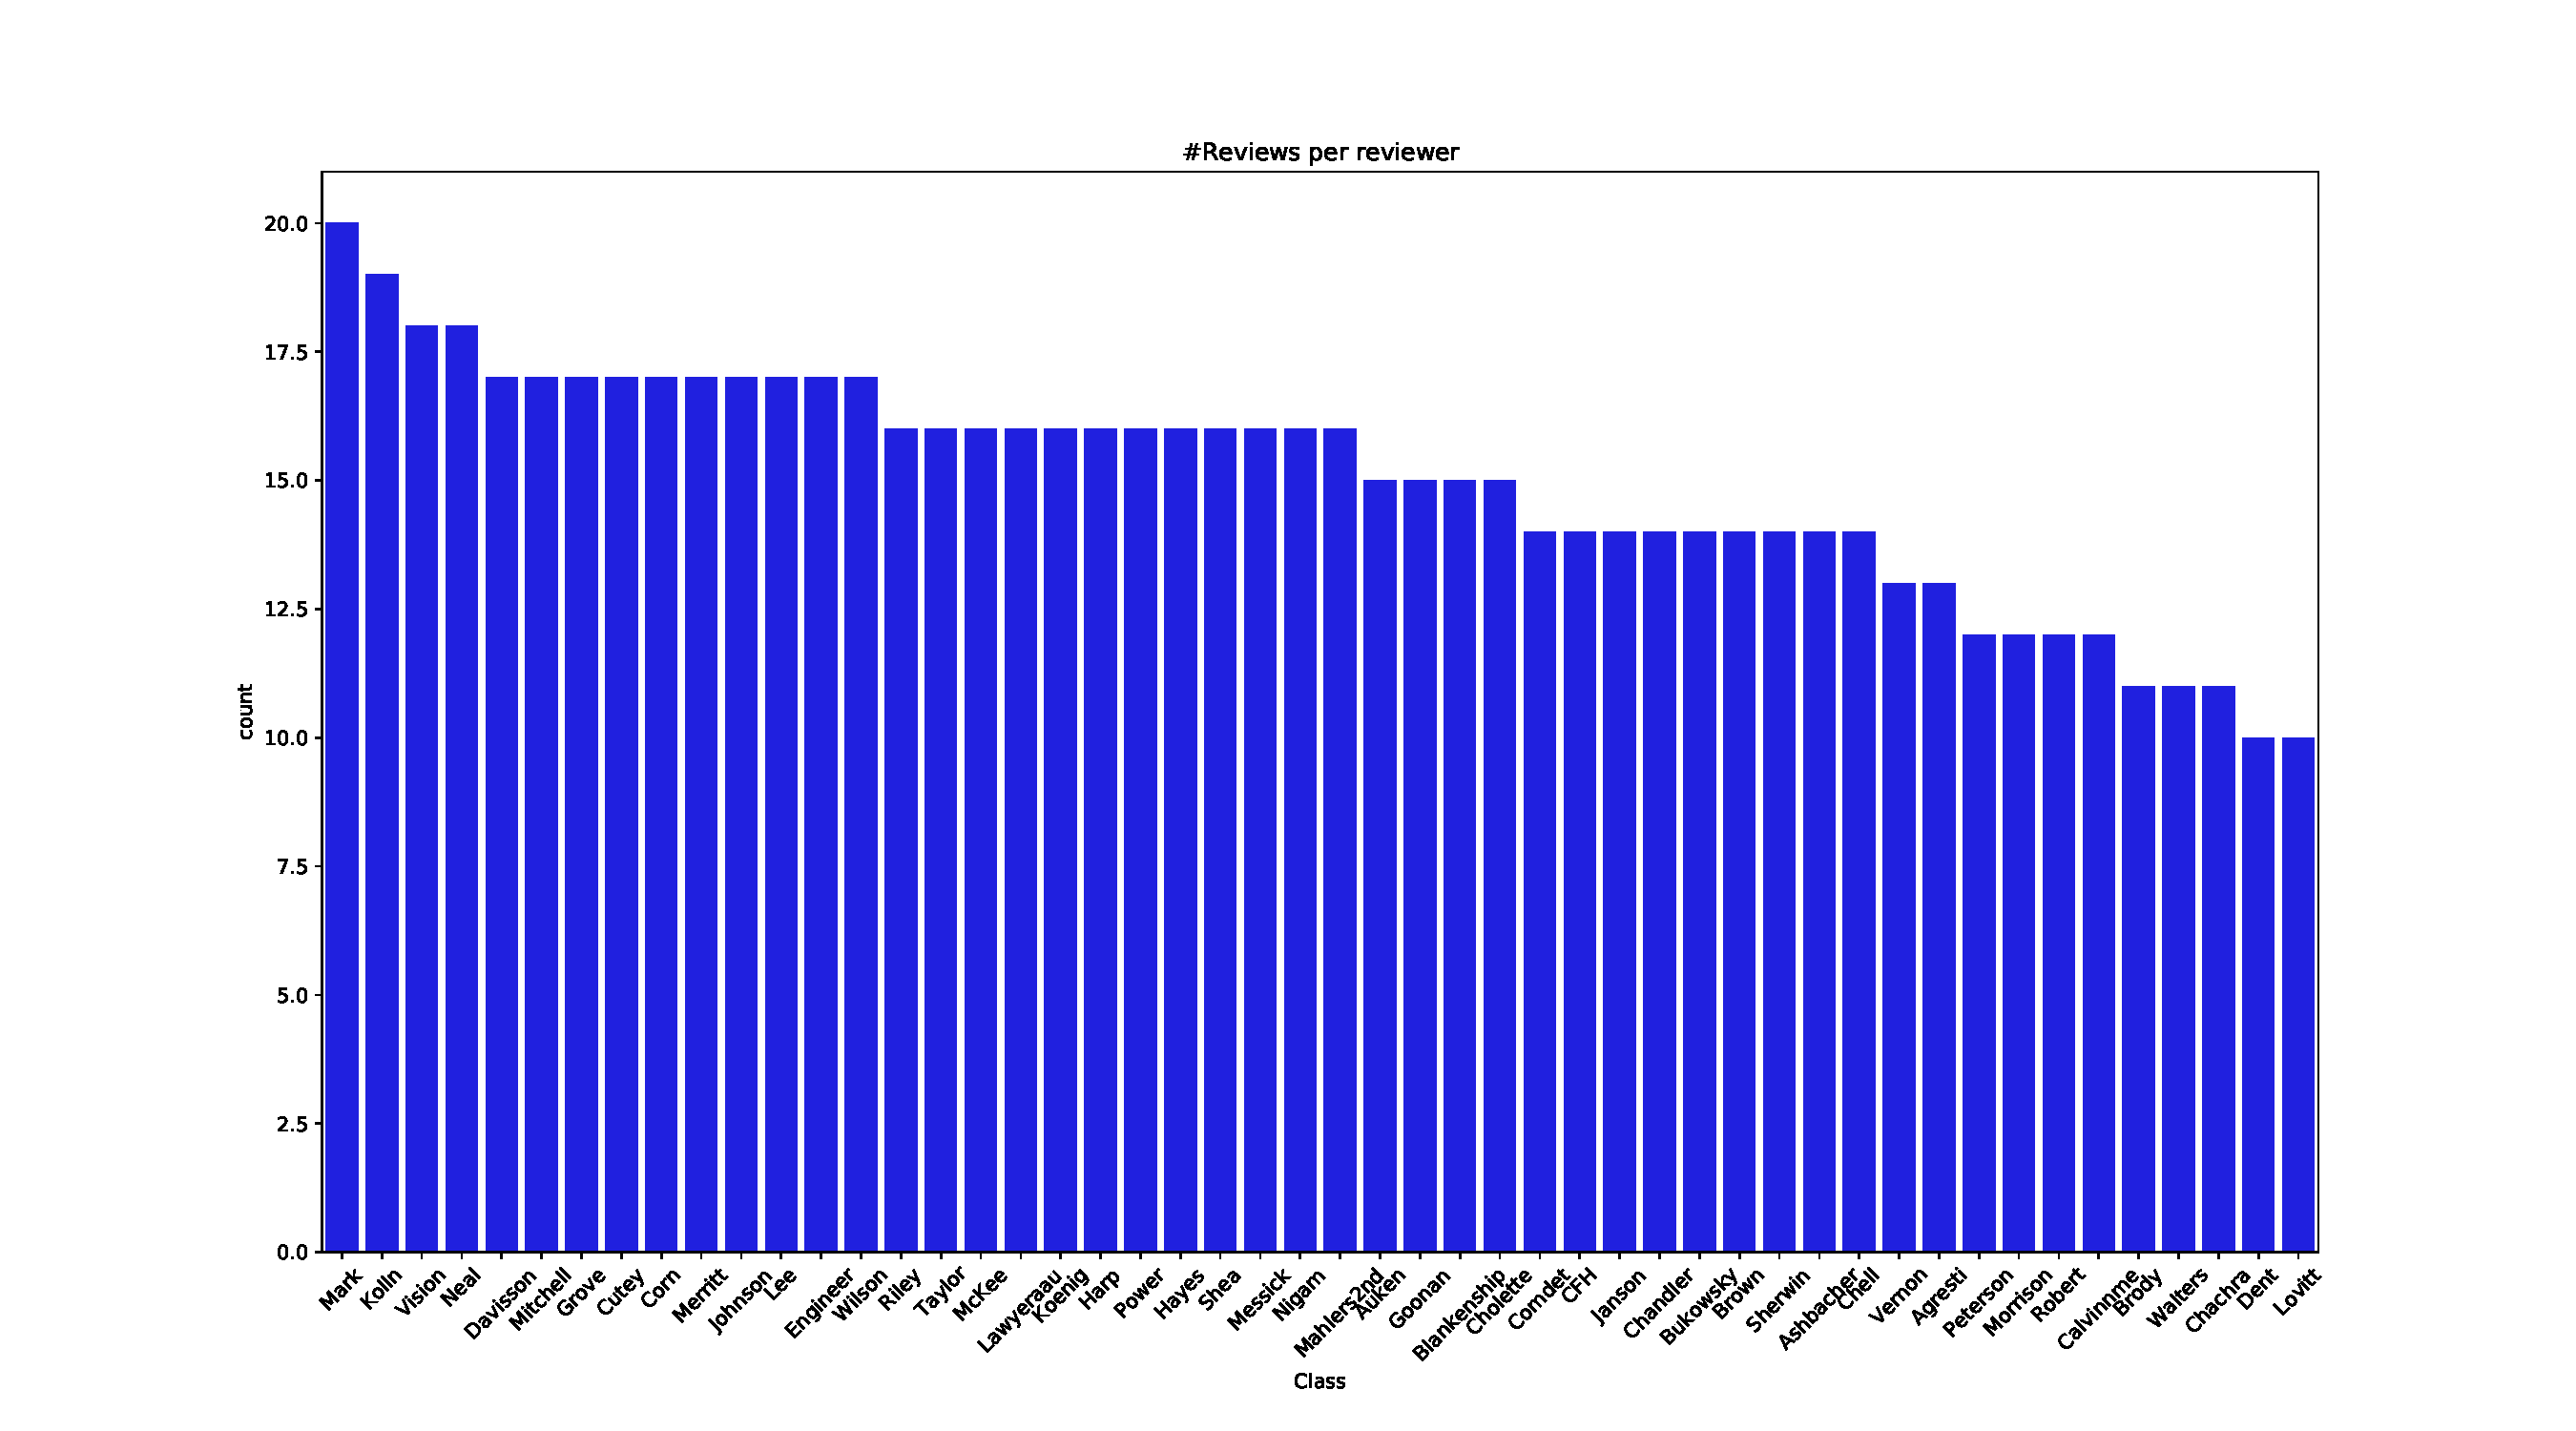
\includegraphics[width=1.0\linewidth]{Instances_per_class.pdf}
%\end{picture}
\end{minipage}
\caption{Instances per class}
\label{Fig::Instances_per_class}
%\end{minipage}
\end{figure}
%
\subsection{Pre-Processing}
There are no missing values in the dataset. The unique ID has been deleted from the data set as has no relevance to the class. The text vectors have values differentiating of a mean of 250 occurrences per instance to 1 occurrence in the entire dataset. With 250 occurrences per instance it appears as though stop words have not been deleted from the dataset, however as we do not have the raw data available we cannot be certain. 
\newline
We sort the vectors from highest number of total occurrences to the smallest number of total occurrences. Words which only occur in one instance can be seen as unique identifier to one author. By sorting the data we enable, to train our model leaving some of the first and last columns out and test whether this improve the model. The different scenarios taken into account can be seen in figure \ref{Fig::Descriptioon of scenarios}
\newline
In figure \ref{Fig::Distribution sum of vectors} one can see the distribution of the sum of the vectors. On average a word appears 309 times in all reviews, however there is a word which appears 187520 times, from 49 to 410 times in a review.
\newline
Two transformations to the dataset have been applied in order to flatten the weight of words which occur more often in one instance. The first transformation is the natural logarithm. The dataset will be transferred into $ln(X)+1$. The one is added to each entry to ensure 0 entries stay 0. The second transformation is a binary translation wher $x_{i,j}=1$ when $x_{i,j}>1$. The scenarios will be ran for both transformations as well.  
%
\begin{figure}
\begin{minipage}[t]{0.3\textwidth}
\begin{tabular}{lr}
\toprule
{} &	Sum of vectors \\
\midrule
count &   10000.000000 \\
mean  &     308.859700 \\
std   &    2419.468303 \\
min   &       0.000000 \\
25\%   &       9.000000 \\
50\%   &      21.000000 \\
75\%   &     220.000000 \\
max   &  187520.000000 \\
\bottomrule
\end{tabular}
\caption{Distribution sum of vectors}
\label{Fig::Distribution sum of vectors}
\end{minipage}
%
\begin{minipage}[t]{0.6\textwidth}
\begin{tabular}{lll}
\toprule
{} &   Scenario &  Scenario description \\
\midrule
0 &      10000 & Select all 10000 attributes   \\
1 &       8000 & select the first 8000 attributes  \\
2 &       6000 & select the first 6000 attributes   \\
3 &   50:10000 & select the 50th till the 10000th attribute   \\
4 &    50:8000 & select the 50th till the 8000th attribute    \\
5 &    50:6000 & select the 50th till the 6000th attribute    \\
6 &  100:10000 & select the 100th till the 10000th attribute    \\
7 &   100:8000 & select the 100th till the 8000th attribute    \\
8 &   100:6000 & select the 100th till the 6000th attribute	\\ 
\bottomrule
\end{tabular}
\caption{Description of different scenarios}
\label{Fig::Descriptioon of scenarios}
\end{minipage}
\end{figure}
%
\subsection{Parameter-Tuning}
First we will split the data in two parts. One part, 90 \%, for training and avlidation of the model with different parameters and the second part, 10\%, to test the models afterwards. To extract the test set, the hold out strategy has been used.
\newline
To split the rest of the data in a training dataset, and a validation dataset, both, the hold out strategy and the cross validation using 10-fold have been used. For the hold out a division of 80\% training and 20\% validation has been 
The results of the model on the validation sets are used to tune the parameters on the model.
\newline
In order to set the scenarios and the parameters used we will make use of the average F1-score. 
%
\newline
\textbf{Perceptron}:We determine the base parameters for the perceptron, alpha as 0.0005, eta as 1 penalty='none' and the max iterations are equal to 100. The results of the 9 scenarios for all tranformations can be found in figures  \ref{Fig::Perceptron parametertuning} using both the hold out and cross validation strategy.
All train sets of the transformed datasets havean F1-score of 100. For the non-transformed dataset a score of 100 was only obtained when high occurring words were deleted.. 
\newline
Comparing the F-1 of the test set of the different transformations binary transformation performs the worse in all scenarios. The logarithmic transformations performs better when we do not delete the words with high occurrences. After removing the top 50 words the F1-score of the $X$ dataset is higher than the$ln(X)+1$ dataset. This can be explained due to the fact that transforming the data into logarithmic values has the highest effect on the words which occur most often.
\newline
A clear difference can be seen between the performance of the hold out and the cross validation runs. The cross validation run has more stable result, where the hold out fluctuates more. Due to the high amount of classes, 50, and the relative low amount of instances it can happen that classes are not represented in the test set, some classes only appear 10 times in the entire dataset. The performance is sensitive to the chosen validation and train set. With using the cross validation the entire dataset is used (except the part left out for testing) and the influence of chance decreases. In order to tune the hyper parameters we will use the cross validation and look at the results of the validation set. Due to the high complexity of the data, and a relative little instances the classifiers can train the model to fit training data exactly, even with linear classifiers. Therefore the results on the training data cannot be compared. 
\newline
For the parameter tuning of on the perceptron classifier scenario 3 of the non-transformed dataset is chosen as it has the best f1-score.
%
\begin{figure}[t]
\begin{minipage}[t]{0.33\textwidth}
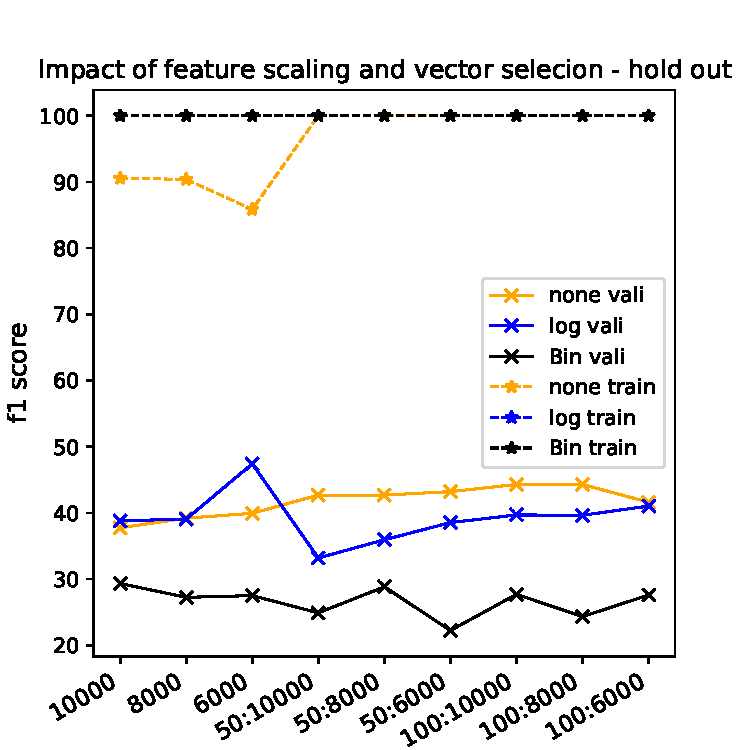
\includegraphics[width=1\linewidth]{perc_scaling_vect_selection_HO.pdf}
\end{minipage}
\begin{minipage}[t]{0.33\textwidth}
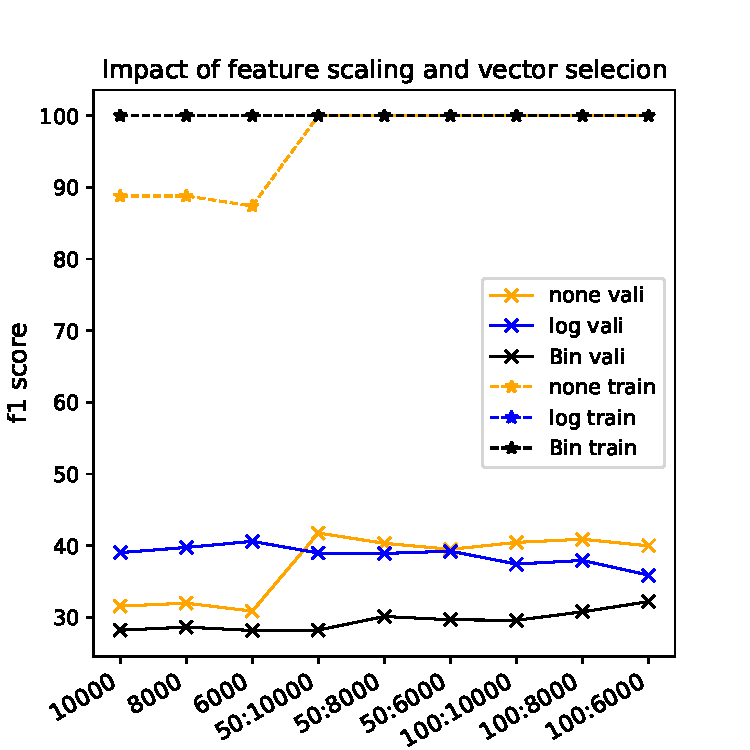
\includegraphics[width=1\linewidth]{perc_scaling_vect_selection.pdf}
\end{minipage}
\begin{minipage}[t]{0.33\textwidth}
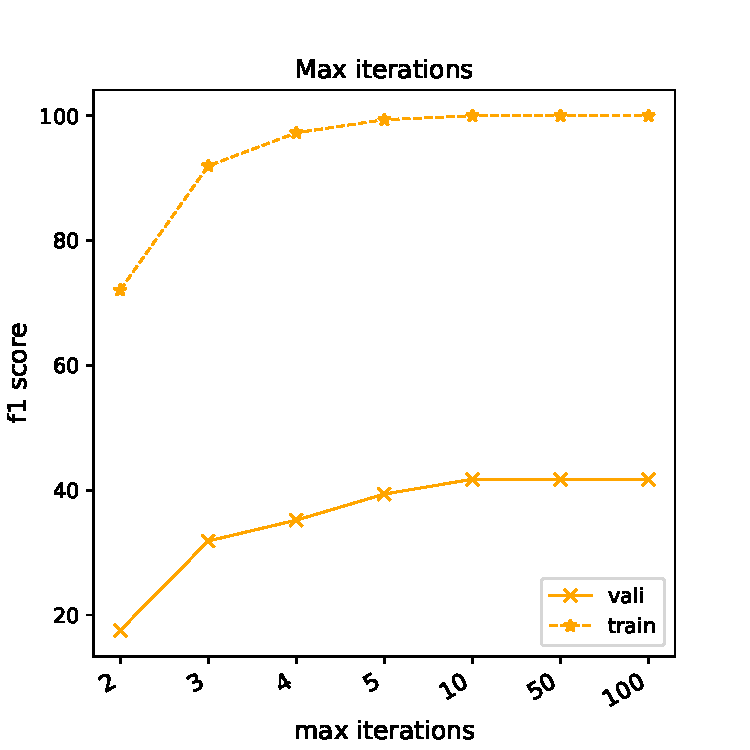
\includegraphics[width=1\linewidth]{Per_max_iterations_2.pdf}
\end{minipage}
\begin{minipage}[t]{0.33\textwidth}
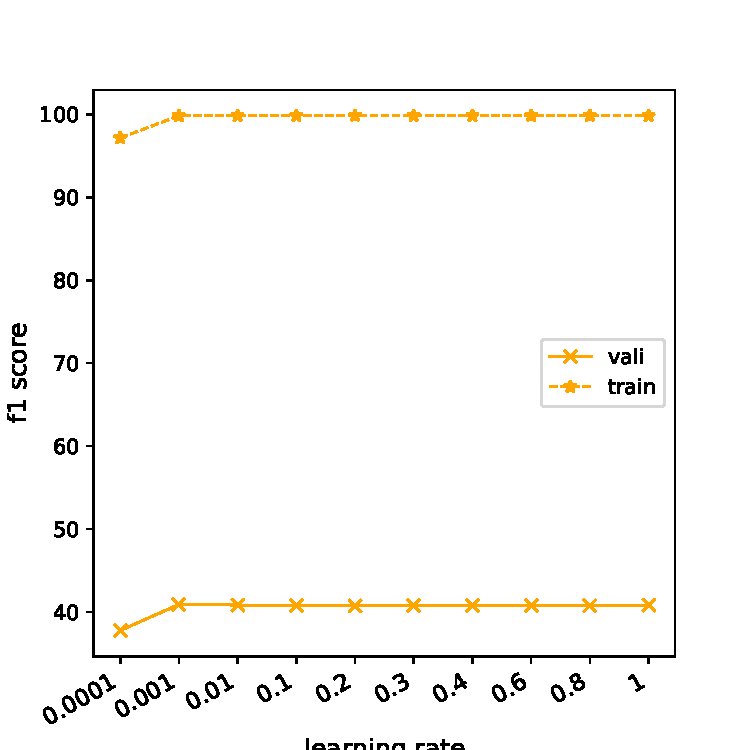
\includegraphics[width=1\linewidth]{Per_learning_rate2.pdf}
\end{minipage}
\begin{minipage}[t]{0.33\textwidth}
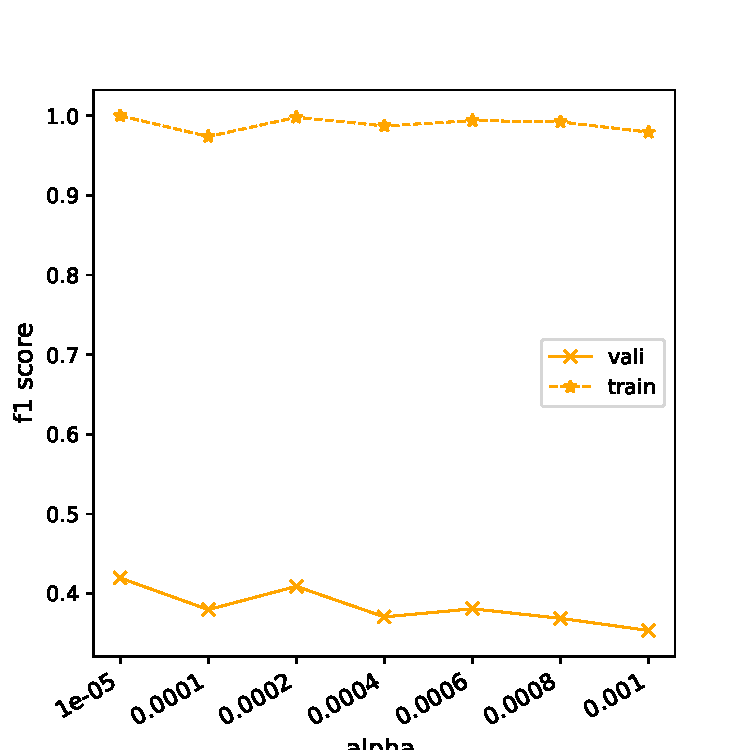
\includegraphics[width=1\linewidth]{Per_alpha2.pdf}
\end{minipage}
\caption{Parameter tuning perceprton}
\label{Fig::Perceptron parametertuning}
\end{figure}
%
The first parameter we tune is the maximum number of iteration maxiter. We test for values  maxiter $\in \{2, 3, 4, 5, 10, 50, 100\}$. It can be seen that after 10 iterations the training set has a perfect fit, and the validation set has the highest performance. Therefore, we take $maxiter=10$ for the next parameter tuning.
\newline
Next the model is trained for different learning rates ($eta0$), where $ eta0 \in \{1^{-4}, 1^{-3}, 0.01, 0.1, 0.2, 0.3, 0.4, 0.6, 0.8, 1\} $. The model is only influences slightly by the different learning rates.The highest performance was obtained wit a learning rate of 0.01. 
\newline
Finally a regularization term has been introduced.We ram $\alpha$ was set to be $ \in \{ 1e^{-4}, 1e^{-3}, 0.01, 0.5, 1\}$. The f1-score for both the training set as well as the validation set dropped rapidly after $1^{-3}$. Therefore, a second run with $\alpha \in  \{1e^{-5}, 1e^{-4}, 0.0002, 0.0004, 0.0006, 0.0008, 1e{-3}\}$ has been done. For $\alpha=0.00001$, the validation performs best with an f1 score of  $42.0\%$. 
%
We run our final model for the test set with the best parameters settings from the parameter tuning. The parameters are as follows maximum number of iterations is 10, $eta0=0.0011$, the regularization term is l1, with an $\alpha$ of $0.00001$ against the test set. This results in an accuracy of $53.3\%$ and a f-1 score of $49.8\%$. 
%
\begin{figure}[t]
\begin{minipage}[t]{0.33\textwidth}
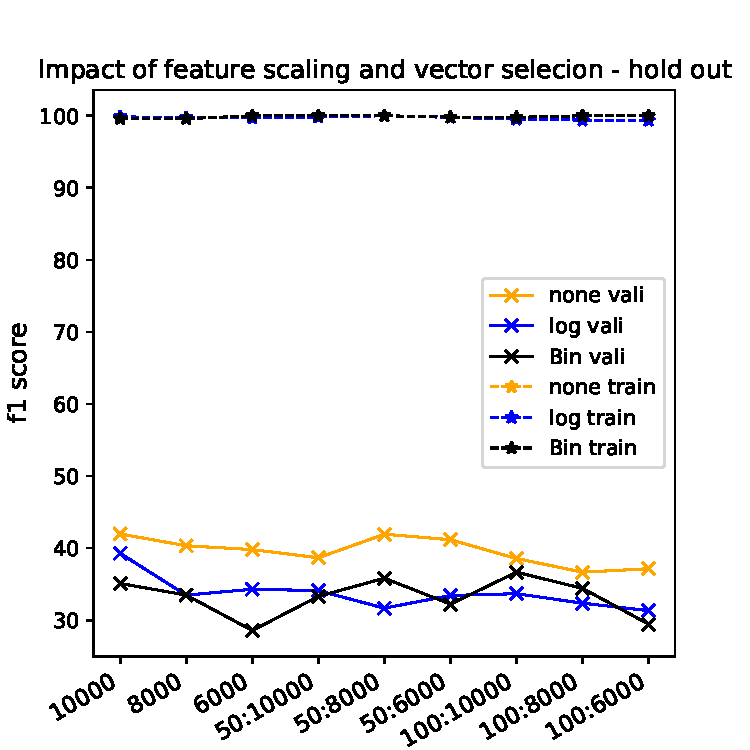
\includegraphics[width=1\linewidth]{RF_scaling_vect_selection_HO.pdf}
\end{minipage}
\begin{minipage}[t]{0.33\textwidth}
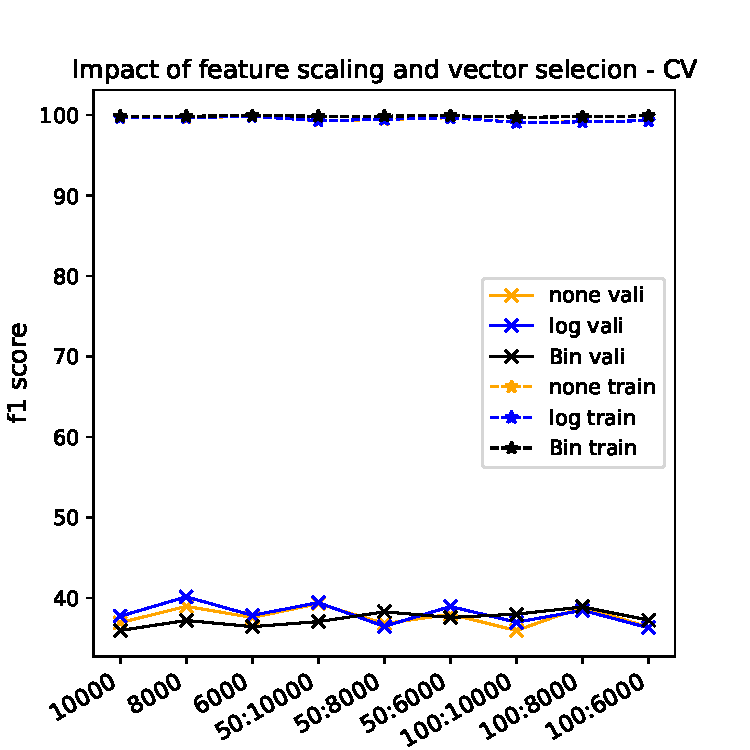
\includegraphics[width=1\linewidth]{RF_scaling_vect_selection_CV.pdf}
\end{minipage}
\begin{minipage}[t]{0.33\textwidth}
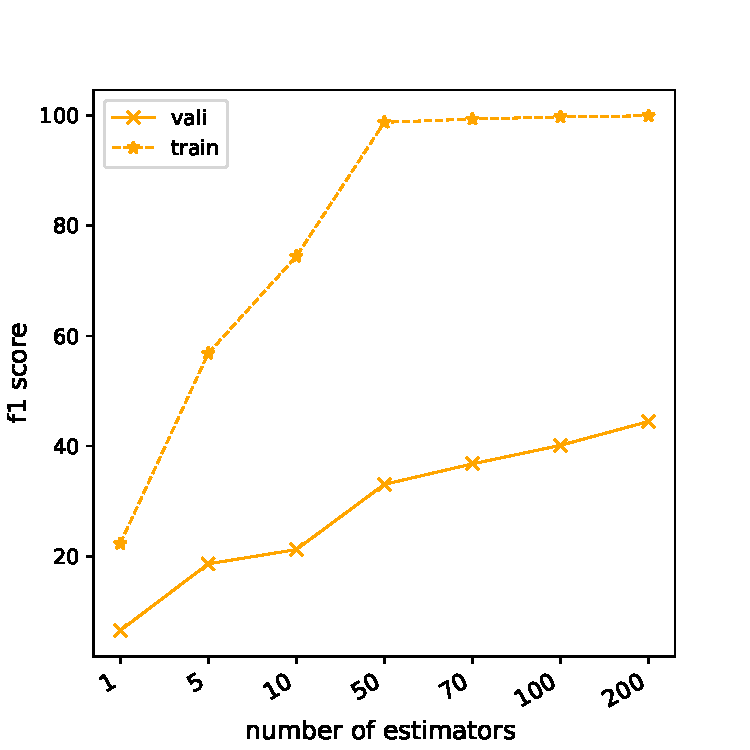
\includegraphics[width=1\linewidth]{RF_nestimators.pdf}
\end{minipage}
\begin{minipage}[t]{0.33\textwidth}
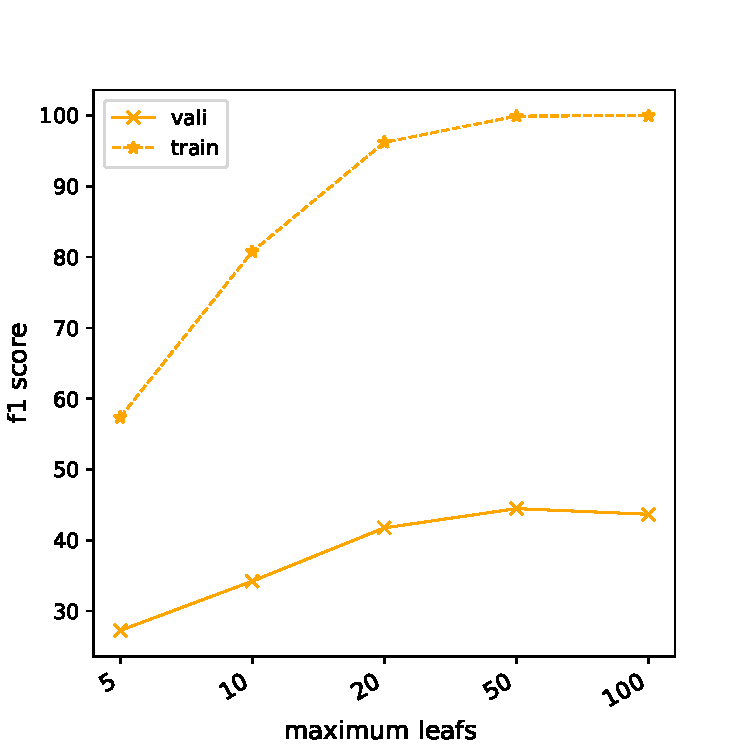
\includegraphics[width=1\linewidth]{RF_max_leafs.pdf}
\end{minipage}
\begin{minipage}[t]{0.33\textwidth}
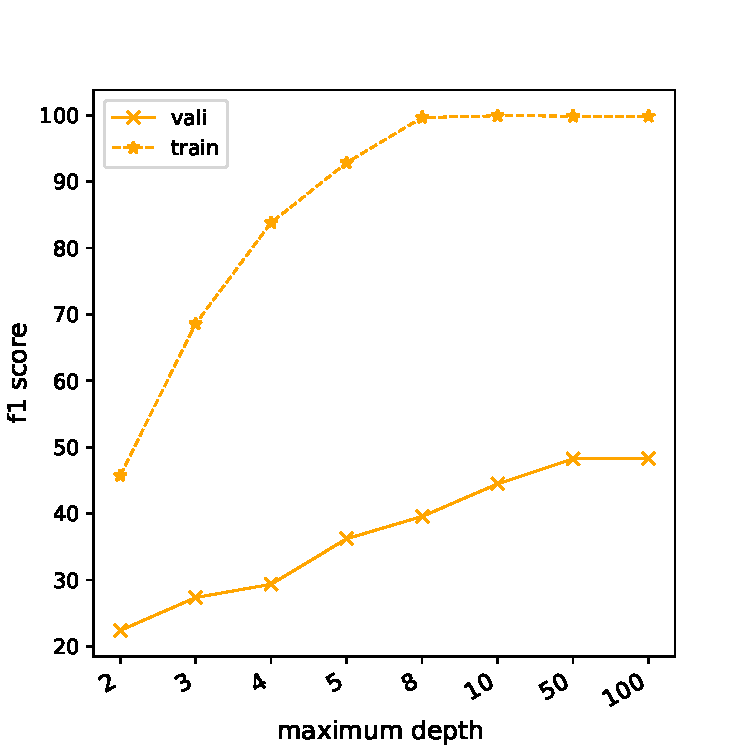
\includegraphics[width=1\linewidth]{RF_max_depth.pdf}
\end{minipage}
\begin{minipage}[t]{0.33\textwidth}
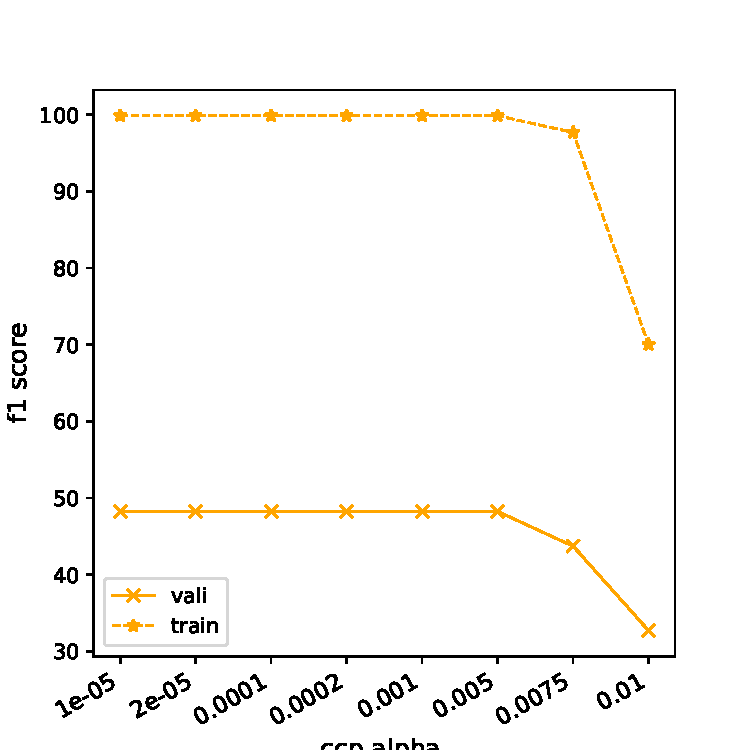
\includegraphics[width=1\linewidth]{RF_ccp_alpha.pdf}
\end{minipage}
\caption{Parameter tuning random forest}
\label{Fig::Random forest parameter tuning}
\end{figure}
%
\newline
\textbf{Random forest}: The second classifier is the random forest classifier. The base parameter settings are the following:$ccp \alpha = 0$, $max leaf = 50$, $max depth = 10$ and
$number of estimators = 100$. The results of the different scenarios for hold out and cross validation can be found in the figures \ref{Fig::Random forest parameter tuning}. The best accuracy is obtained scenario 2 on the natural logarithmic dataset with an f1-score of $40.15\%$ in the cross validation. For the first scenarios the logarithmic transformation performs best. Starting at scenario 4 the performances come closer together and there is no transformation which out performs the other. 
\newline
The following hyper parameters have been tested: number of estimators, the maximum depth, maximum leafs and the complexity cost parameter, ccp alpha. Starting with the number of estimators, the number of trees, given n estimators $\in \{1,5,10, 50, 70, 100, 200\}$. 
\newline
Both the train set and the validation set achieve an higher performance, for all scoring methods, whenever the number of estimators increases. The number of estimators is set to 200.
\newline
The second hyper parameter is the maximum number of leafs per branch, we test $max leafs \in \{5,10, 20, 50, 100\}$ The accuracy increases when the number of leafs increase to 50, with 100 all performances increase for the training set, but not for the test set. The model is over fitting. The maximum number of leafs is set to 50.   
\newline
After the number of trees and the leafs per branch, the depth of each tree is determined. where $max depth \in \{2, 3, 4, 5, 8, 10, 50, 100\}$. The f1-score for the training set is highest with a maximum depth of $10$. The f1-score for the validation set is highest with a maximum depth of $50$ or a $100$, the same scores are obtained. The maximum depth is set to $50$. 
\newline
Last, we tune the minimal cost complexity pruning parameter. We test for $ccp  \alpha \in \{1e-5, 2e-5, 1e-4, 2e-4, 1e-3, 5e-3, 75e-4, 1e-2\}$. It can be seen that for $ccp \alpha < 0.005$ the pruning does not cost. However, for $ccp \alpha > 0.005$ both the train and the test have reduced scores. Therefor, we will set $ccp \alpha=0.005$.   
%
The final model is now tested on the validation data with the following parameter settings:
$n estimators = 200$ ,$max_leaf = 50$, $max_depth = 50$ and $ccp \alpha = 0.005$. This results in an f1-score of $51.8\%$.
\newline 
\textbf{Naive Bayes}: The third classifier is the multinominal Naive Bayes classifier. For the base run we set $\alpha$ equal to 1. The nine scenarios are run for both hold out and cross validation. A clear pattern can be seen in the result. The accuracy of the non transformed dataset clearly out performs the logarithmic and the binary transformations. Furthermore it can be seen that including less vectors improves the model, both the first and the last vectors from the dataset. As the best results are obtained in scenario 8, additional scenarios are ran excluding additional vectors from the beginning and the end.  
\newline
First 5 additional scenarios are created excluding more vectors in the end. The best results are obtained with scenario 11, and 12. Another 10 scenarios are considered leaving the first 150, 200, 250, 300 and 350 vectors out until the 4000th and the 4500th vector. The accuracy can be found in table \ref{Fig::Naive Bayes parameter tuning}. the best accuracy is obtained in scenario 250 closely followed by scenario 22.
\newline
The first 9 scenarios have been ran for different smoothing priors. We ran the model for alpha's $\in \{1e{-3}, 1e{-2}, 1e{-1}, 0.5, 1, 10, 100, 1000\}$. All results are equal for all alphas.  
\begin{figure}[h]
\begin{minipage}[t]{0.33\textwidth}
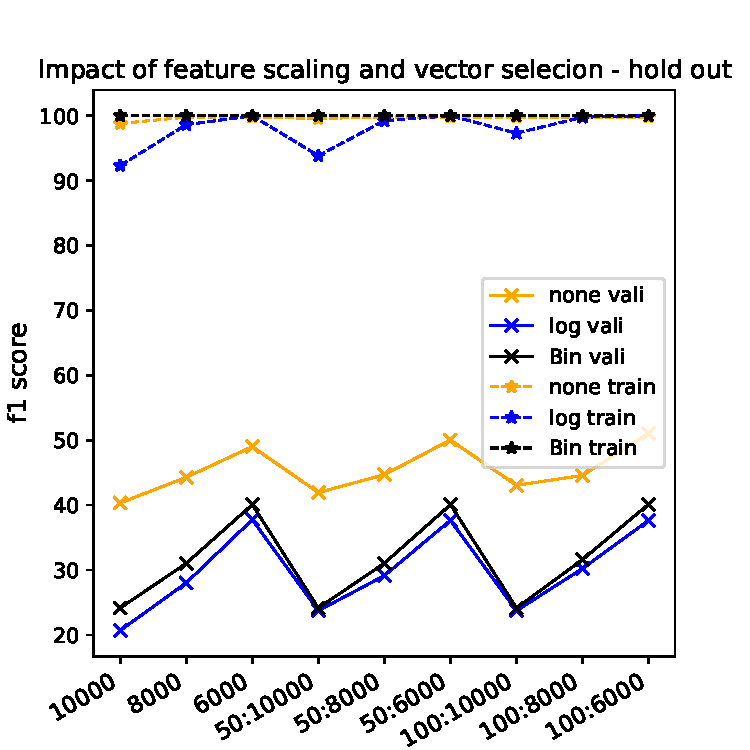
\includegraphics[width=1\linewidth]{NB_scaling_vect_selection_HO.pdf}
\end{minipage}
\begin{minipage}[t]{0.33\textwidth}
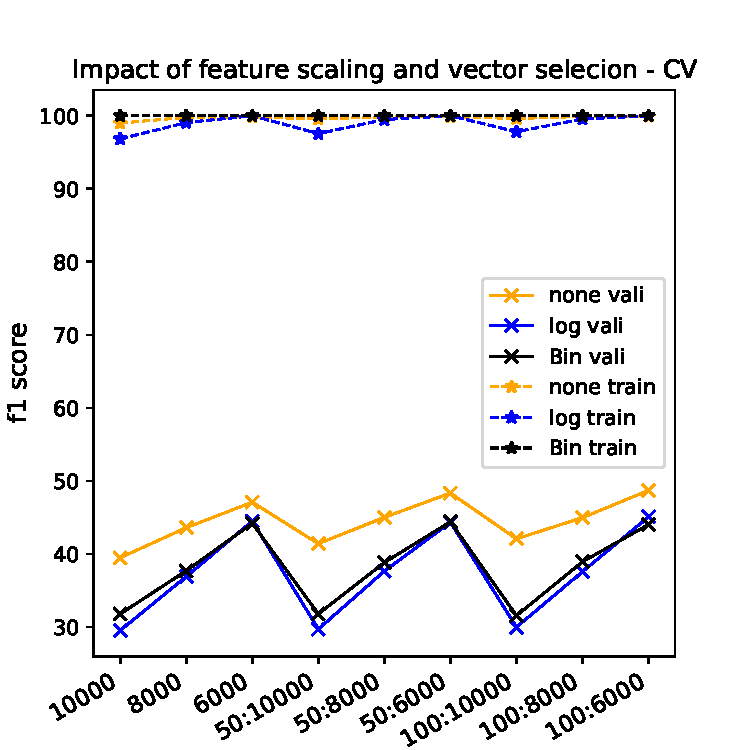
\includegraphics[width=1\linewidth]{NB_scaling_vect_selection_CV.pdf}
\end{minipage}
\begin{minipage}[t]{0.33\textwidth}
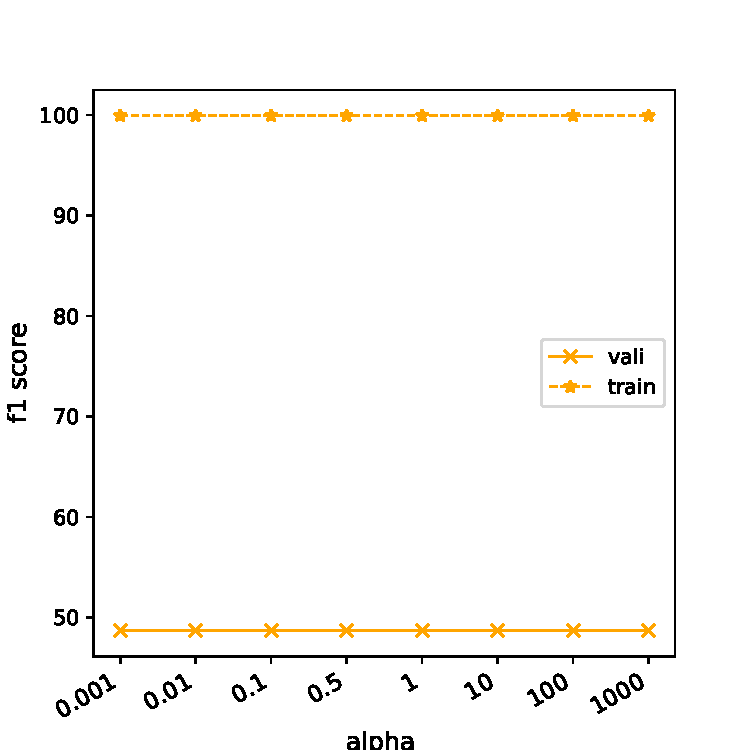
\includegraphics[width=1\linewidth]{NB_alpha.pdf}
\end{minipage}
\begin{minipage}[t]{0.33\textwidth}
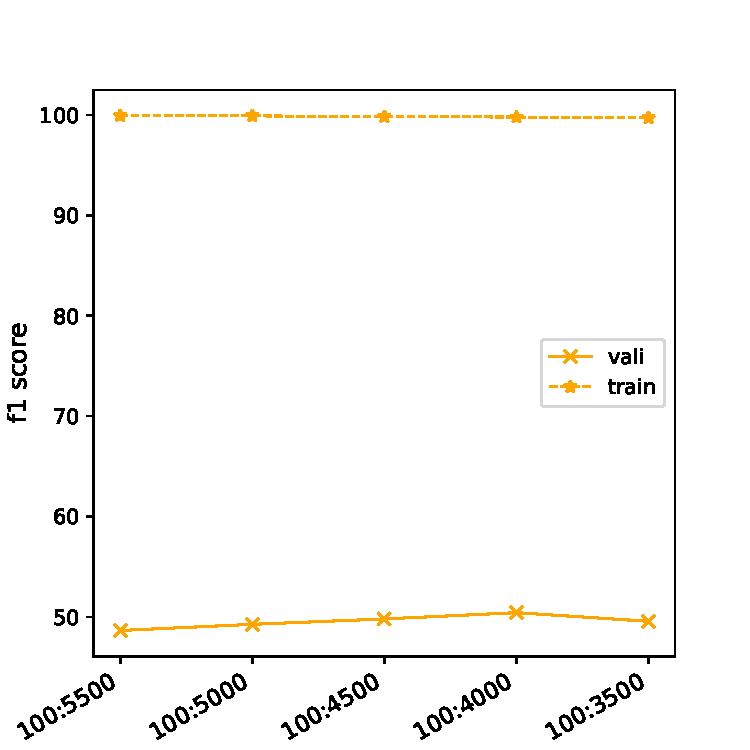
\includegraphics[width=1\linewidth]{NB_Xrange2.pdf}
\end{minipage}
\begin{minipage}[t]{0.33\textwidth}
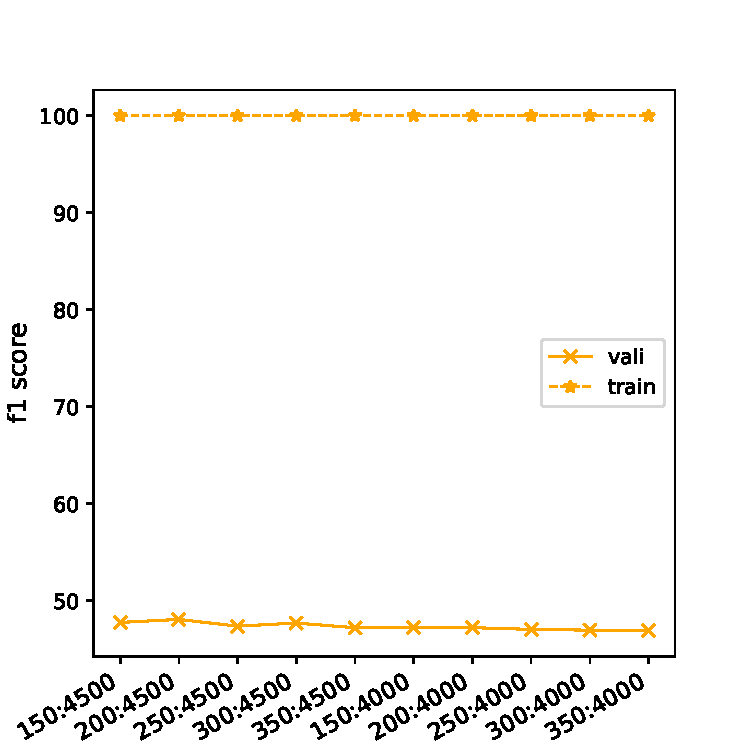
\includegraphics[width=1\linewidth]{NB_Xrange3.pdf}
\end{minipage}
\begin{minipage}[t]{0.33\textwidth}
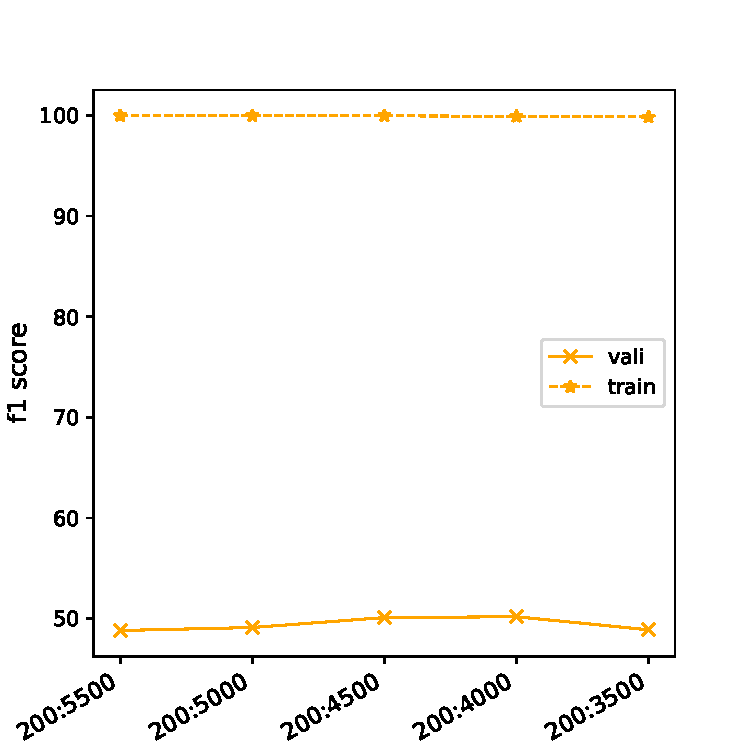
\includegraphics[width=1\linewidth]{NB_Xrange4.pdf}
\end{minipage}
\caption{Parameter tuning Naive Bayes.}
\label{Fig::Naive Bayes parameter tuning}
\end{figure}

\section{Bridges Dataset(\href{https://archive.ics.uci.edu/ml/datasets/Pittsburgh+Bridges}{link to dataset})}


\end{document}


